% !TEX TS-program = pdflatex
% !TEX encoding = UTF-8 Unicode
%% For double-blind review submission
\documentclass[acmsmall,screen]{acmart}\settopmatter{printfolios=true}
%% For single-blind review submission
%\documentclass[acmlarge,review]{acmart}\settopmatter{printfolios=true}
%% For final camera-ready submission
%\documentclass[acmlarge]{acmart}\settopmatter{}

%% Note: Authors migrating a paper from PACMPL format to traditional
%% SIGPLAN proceedings format should change 'acmlarge' to
%% 'sigplan,10pt'.


%% Some recommended packages.
\usepackage{booktabs}   %% For formal tables:
                        %% http://ctan.org/pkg/booktabs
\usepackage{subcaption} %% For complex figures with subfigures/subcaptions
                        %% http://ctan.org/pkg/subcaption


\makeatletter\if@ACM@journal\makeatother
%\acmDOI{10.1145/nnnnnnn.nnnnnnn}
\startPage{1}
\else\makeatother
%% Conference information (used by SIGPLAN proceedings format)
%% Supplied to authors by publisher for camera-ready submission
%\acmDOI{10.1145/nnnnnnn.nnnnnnn}
\startPage{1}
\fi


%% Copyright information
%% Supplied to authors (based on authors' rights management selection;
%% see authors.acm.org) by publisher for camera-ready submission

%% Bibliography style
\bibliographystyle{ACM-Reference-Format}
%% Citation style
%% Note: author/year citations are required for papers published as an
%% issue of PACMPL.
\citestyle{acmauthoryear}   %% For author/year citations

\usepackage{uri}
\usepackage{mathtools}
\usepackage{amsthm}
\usepackage{mathpartir}
\usepackage{semantic}
\usepackage{graphicx}
\usepackage{cases}
\usepackage{hyperref}
\usepackage{stmaryrd}
\usepackage{listings}
\usepackage{iris}
%\usepackage{lstlangcoq}
\renewcommand{\lstlistingname}{Figure}

\clubpenalty = 10000
\widowpenalty = 10000
\displaywidowpenalty = 10000

\lstset{language=C,basicstyle=\ttfamily,mathescape=true,columns=fullflexible}

\newcommand{\TODO}[1]{\textbf{\textcolor{red}{[ TODO: #1]}}}
%\newcommand{\boxdotright}{\!\mathrel\boxdot\joinrel\rightarrow\!}
\newcommand{\islock}{\boxdotright}
\newcommand{\isaex}{\!\mathrel\odot\joinrel\rightarrow\!}
\newcommand{\xisaex}[1]{\!\mathrel\odot\joinrel\xrightarrow{#1}\!}
%% \newcommand{\ifthenelse}[3]{\text{if }#1\text{ then }#2\text{ else }#3}
\newcommand{\emp}{\mathsf{emp}}

\newcommand\dboxed[1]{\dbox{\ensuremath{#1}}}
\newcommand{\master}[2]{\ensuremath{\mathrm{Master}_{#1}(#2)}}
\newcommand{\snap}[1]{\ensuremath{\mathrm{Snapshot}(#1)}}
\newcommand{\ghost}[2]{\ensuremath{\dboxed{#1}^{#2}}}
\newcommand{\us}{$\mu$s}
\newcommand{\gnamety}{\ensuremath{\mathsf{gname}}}
\newcommand{\treerep}{\ensuremath{\mathsf{bst}}}
\newcommand{\nodeboxrep}{\ensuremath{\mathsf{bst\_ref}}}

\newcommand{\ignore}[1]{}

\hyphenation{Comp-Cert}

\usepackage[utf8]{inputenc}
\usepackage{geometry}
\geometry{a4paper}

\usepackage{graphicx} % support the \includegraphics command and options
\usepackage{verbatim} % adds environment for commenting out blocks of text & for better verbatim
%\usepackage{amssymb}
\usepackage{url}
\usepackage{listings}

\title{Verifying Fine-Grained and Lock-Free Binary Search Trees}
\author{Roshan Sharma}
\author{Shengyi Wang}
\author{Alexander Oey}
\author{Lennart Beringer}
\author{William Mansky}

\date{} % Activate to display a given date or no date (if empty),
         % otherwise the current date is printed 

\begin{document}
\acmConference{Some conference}
\maketitle

\catcode`\@=11
\section{Introduction}
The binary search tree (BST) is a common implementation of an ordered
map, a widely used data structure. The concurrent version of the
ordered map forms the bedrock of many parallel programs. We formally
verified the functional correctness of two versions of fine-grained
concurrent binary search trees (CBST) written in C. One adopts the
hand-over-hand locking technique \cite{bayer1977}, the other is lock
free by using atomic primitives such as compare and swap (CAS). Both
CBST implementations support insert, lookup, and delete operations; %or do we have lock-free without delete?
they also share the ``same'' specifications to some extent in our
verification. All the proof is machine-checked in Coq. %Say something about existing proofs of fine-grained data structures and how we compare.

Our specifications use the logical atomicity introduced in the TaDA
logic \cite{tada}, in the form of \emph{atomic Hoare
triples}. Intuitively, an atomic Hoare triple $ \langle
P \rangle\,\mathbb{C}\, \langle Q \rangle$ means the program
$\mathbb{C}$ ``atomically updates'' from $P$ to $Q$. The program may
actually take multiple steps, but every step before the atomic update
(linearization point) must preserve the assertion $P$. Meanwhile, the
concurrent environment may also update the state before the
linearization point, as long as the states satisfies $P$. The
assertion $Q$ must become true at the linearization point, then the
environment can do whatever it likes. There is no guarantee that $Q$
is still preserved when $\mathbb{C}$ returns. For example, the
specification of our \texttt{insert} operation may be explained as
follows: during the execution of \texttt{insert}, there is
always \emph{some} BST, and at some point the \texttt{insert} will
take a BST $t$, insert a value with a certain key, and then eventually
returns (meanwhile other threads may have further modified the
inserted tree)\footnote{Maybe say what a reasonable $Q$ is and why such a spec is still useful, specifically w.r.t. the situation where one of the other threads' action following the linearization point removes the element just inserted.}.

We employ the Verified Software Toolchain (VST) \cite{plfcc} to verify
the correctness of CBST. Although the concurrent separation logic
(CSL) has been formalized in VST rooted on the work of Hobor et
al.\ \cite{oraclesematic}, we extend it with two descendants of CSL so
as to accomplish the verification. One is the logical atomicity
mentioned above; the other is the higher-order ghost state in the
style of Iris \cite{higherorderghoststate}. The ghost states are used
to contruct both the global invariants and the local state in our
proofs. They will be further discussed in \S\ref{correctness}.

We highlight a few innovative aspects of our verification of CBST:
\begin{description}
\item [Range ghost] We abstract the BST via a pair of values
called \emph{range} which represents the lower-bound and upper-bound
of keys on each node to reason about the BST in the current
settings. We prove that range with the merging operation forms a
partial commutative monoid (PCM) so that it can be encoded in ghost
states.

\item [\textsf{sync\_inv} pattern] It is a particular approach
combining locks with general invariants to solve the dilemma caused by
the fine-grained locking mechanism: we do not have a lock to control
the access of the entire BST nor can we access the state of the BST
via atomic operations.
\end{description}

%% Do we have contributions, and are they sufficient? Range ghost is adapted from flow interfaces. Sync_inv pattern isn't totally ours, though it might be instructive w.r.t. combining traditional and Iris-style CSLs, and it might be worth explaining in more detail. We're working on "actual" code, but missing a few pieces to make our proofs foundational. (but maybe it's worth highlighting the extra work we do to work on actual code) We could promote this as the first working example of Iris+VST. We don't yet have any demonstrations on larger or interesting data structures, and this alone was quite a bit of work. The delete logic is rather interesting. Nothing to say about flow interfaces yet, but maybe soon.


Our specific contributions are:
\begin{itemize}
\item To the best of our knowledge, this is the first mechanized
verification of an concurrent search-based data structure written in a
real programming language. %should probably clarify what we mean by "real"

\item We illustrate how to incorporate the CSL in VST, the higher-order
ghost state in the style of Iris, and the logical atomicity from the
TaDA logic together to verify the CBST.
\end{itemize}

We introduce the background about the verification of concurrent C
programs in \S\ref{background}, including the tool-chain VST and Iris,
the concept of ghost states, global invariants, and atomic
specifications. The thread-safety proofs of operations on CBST are
first explained in \S\ref{safety}, where we show the \emph{recursive}
lock pattern for hand-over-hand locking mechanism. The functional
correctness proofs are presented in \S\ref{correctness}. We detail the
use of the \textsf{sync\_inv} pattern, the combination of recursive
lock invariants and ghost states together in the atomic
specifications, and the proof skeleton of each operation on CBST. The
related work is discussed in \S\ref{related}. We end with the
conclusion of our work in \S\ref{conclusion}.



\section{Background}
\label{background}
\subsection{VST and Iris}
We use the Verified Software Toolchain \cite{plfcc}  to prove the correctness of the concurrent binary search tree. VST is a Coq-based proof system that helps to prove separation logic properties of C programs with the assurance that the properties will be preserved in compiled code. First, we write programs in C programming and using CompCert’s \emph{clightgen}, the ASTs for C programs can be generated in Coq. We then state and prove specifications for them using Verifiable C. Verifiable C is a higher-order separation logic for reasoning about the functional correctness of C programs and carries a soundness proof that links high-level specifications to assembly code generated by the CompCert Verified compiler. Verifiable C supports reasoning about two separate kinds of concurrency:  Pthreads-style concurrency with locks (used by implementing blocking data structures that can be fine-grained or coarse-grained ), and concurrency using C11 atomic operations (i.e. lock-free data structures). 

\subsection{Ghost State and Global Invariants}
We can prove memory safety and race freedom properties of shared-memory concurrent programs, by tracking the transfer of ownership of shared locations between threads that would happen if we ran the program. But, this idea is insufficient to prove that concurrently running threads are successful to accomplish some task, which is also called functional correctness. For instance, we can prove the memory safety properties of the increment example in  \ref{figure1} through the transfer of ownership of shared variable $x$ between threads. But, we can not guarantee that the value of $x$ will be $2$ after all threads complete their execution, which is demonstrated in \ref{figure1} using separation logic assertion.   
\begin{figure}[htb]
\centering
$\texttt{x = 0;}$\\
$\mathit{I_{\pi}(x \mapsto v \land v \geq 0)}\qquad\pi = \pi_1\ .\ \pi_2$\\
$\begin{array}{l || l}
\mathit{I_{\pi_1}(x \mapsto v \land v \geq 0)} & \mathit{I_{\pi_2}(x \mapsto v \land v \geq 0)}\\
\texttt{acquire(l);} & \texttt{acquire(l);}\\
\mathit{x \mapsto v \land I_{\pi_1}(x \mapsto v \land v \geq 0)} & \mathit{x \mapsto v \land I_{\pi_2}(x \mapsto v \land v \geq 0)}\\
\texttt{x++;} & \texttt{x++;}\\
\mathit{x \mapsto v+1 \land I_{\pi_1}(x \mapsto v \land v \geq 0)} & \mathit{x \mapsto v+1 \land I_{\pi_2}(x \mapsto v \land v \geq 0)}\\
\texttt{release(l);} & \texttt{release(l);}\\
\mathit{I_{\pi_1}(x \mapsto v \land v \geq 0)} & \mathit{I_{\pi_2}(x \mapsto v \land v \geq 0)}\\
\end{array}$\\
$\mathit{I_{\pi}(x \mapsto v \land v \geq 0)}$
\caption{The increment example annotated with separation logic assertion}
\label{figure1}
\end{figure}
We must preserve the connection between the value of shared resources and the work performed by each thread. A common approach to achieve this is to use \emph{ghost variables}, an auxiliary state introduced later in the proof to track the local information about each thread. They do not appear in the original program. Program in \ref{figure1} can be verified by creating ghost state, which tracks the latest action performed by a thread, for each thread with initial value of $0$, and update with $1$ after each thread increment the value of \texttt{x}. In VST, we can create \emph{ghost state} for any Coq type in the form of an arbitrary \emph{partial commutative monoid} (PCM), a set with a partially defined binary operation that is as associative as it can, commutative, and has a unit, as long as we can describe what happens when two elements of that type are joined together. VST provides $\mathsf {ghost\_var}$ assertion to create a simple ghost state: $\mathsf{ghost\_var}\ \mathit{sh}\ a\ g$ asserts that $g$ is a \emph{ghost name} ($\gnamety$ in Coq) associated with the value $a$, which may be of any type. We will see different kind of ghost states used to verify binary search tree in the following sections.

The main idea behind the logic from Iris \cite{higherorderghoststate}, a mechnized higher-order concurrent separation logic framework, is the construction of \emph{global invariant} as \emph{ghost state}. \emph{Global Invariant} is an invariant on the global (ghost and physical) state of program. We can open any invariant but must close it again before taking any steps of execution unless those execution are atomic. Thread can use the contents of \emph{global invariant} during atomic operation if it can guarantee that no one will ever see an intermediate state in which invariant does not hold. The rules from Jung et al.\cite{higherorderghoststate} for creating and opening invariants are:

\begin{mathpar}
\inference[\textsf{inv\_alloc}]{}{\triangleright P \vdash \pvs[E] \mathsf{EX}\ i : \mathsf{iname}, \knowInv{i}{P}}

\inference[\textsf{inv\_open}]{i \in E}{\knowInv{i}{P} \vdash \pvs[E][E \setminus i] \triangleright P * (\triangleright P \wand \pvs[E \setminus i][E] \mathsf{emp})}
\end{mathpar}

where invariants are provided in the form of assertion $\knowInv{i}{P}$, and states that $P$ is maintained as an invariant on the global state with name $i$. The operator%%  $\pvs[][]$
is called ``fancy update" operator,that allows to allocate, open, and close the invariants and the later $\triangleright$ operator is used for impredicativity (i.e. $\knowInv{i}{..\knowInv{i}{P}..}$).

\subsection{Atomic Specifications}
\label{atomic}
For many concurrent data structures, the ideal correctness condition is that the data structure behaves the same as a sequential implementation, even when accessed simultaneously by multiple threads. This intuitive condition can be formalized as linearizability (operations appear to take effect in some total order) or atomicity (client threads never observe intermediate states of operations). In separation logic, atomicity can be expressed in the form of \emph{atomic triples}~\cite{tada}, written in the form $\forall a.\ \langle P_l\ |\ P_p(a)\rangle\ c\ \langle Q_l\ |\ Q_p(a)\rangle$, where $P_l$ and $Q_l$ are \emph{private} pre- and postconditions similar to an ordinary Hoare triple, and $P_p$ and $Q_p$ are \emph{public} pre- and postconditions, parameterized by an abstract value $a$ of the shared data structure. Intuitively, $P_l$ and $Q_l$ must be true before and after the call, while $P_p$ must be true for some value of $a$ at every point from the beginning of $c$ until some designated linearization point, at which point $Q_p$ becomes true atomically for the same value $a$. For instance, the specification $$\forall s.\ \langle \mathsf{is\_stack}\ p\ |\ \mathsf{stack}\ s\rangle\ \texttt{push}(v)\ \langle \mathsf{is\_stack}\ p\ |\ \mathsf{stack}\ (v :: s)\rangle$$ expresses the fact that the \texttt{push} operation of a concurrent stack correctly implements the behavior of a sequential push, atomically transitioning from some stack $s$ to $v :: s$ at some point during its execution. %maybe something about linking ghost state, which parts are real vs. ghost, accessing invariants around atomic triple

VST has encoded an atomic Hoare triple, and provide the way that matches the notation VST uses for normal specifications. Such specification is called \emph{atomic specification}, and can be formalized in Coq as shown in  \ref{atomic-spec}.  This is how we write pre- and postcondition in VST. 
\begin{figure}[htb]
\centering
\begin{verbatim}
Program Definition insert_spec :=
DECLARE _insert
ATOMIC TYPE W OBJ a INVS Ei Eo
WITH ...
PRE [ ... ]
  PROP (...)
  LOCAL (...)
  SEP (P_l) | (P_p)
POST [ ... ]
  PROP ()
  LOCAL ()
  SEP (Q_l) | (Q_p)
\end{verbatim}
\caption{Atomic Specification in VST}
\label{atomic-spec}
\end{figure}
\texttt{W} is the \textsf{TypeTree} representing the type of arguments passed with \texttt{WITH} clause; \texttt{a} is the abstract state for the triple; \texttt{Ei} and \texttt{Eo} are the sets of invariants names inside and outside the triple. The \texttt{PROP} clause describes things that that are true independent of program state, the \texttt{LOCAL} clause describes the values contained in C local variables, and the \texttt{SEP} clause represents the \emph{separating conjunction} (*) of \emph{spatial predicates}, predicates on some part of the memory. In VST, while proving that a function implements an atomic specification, the precondition will contains an $\mathsf{atomic\_shift}$ assertion with the public pre- and postcondition, and the masks inside it. This atomic shift can be accessed through following two rules:
$$\inference[\textsf{atomic\_commit}]{\forall a, R * P_p\ a \Rrightarrow \mathsf{EX}\ y,\ Q_p\ a\ y * R'\ y}{\textsf{atomic\_shift}(P_p, E_i, E_o, Q_p, Q) * R \Rrightarrow \mathsf{EX}\ y,\ Q\ y * R'\ y}$$
$$\inference[\textsf{atomic\_rollback}]{\forall a, R * P_p\ a \Rrightarrow P_p\ a * R'}{\textsf{atomic\_shift}(P_p, E_i, E_o, Q_p, Q) * R \Rrightarrow \textsf{atomic\_shift}(P_p, E_i, E_o, Q_p, Q) * R'}$$
During commit, we must provide resources $R$ which, in combination with the public precondition $P_p$, allow us to prove the public postcondition $Q_p$. Then, we gain access to an assertion $Q$ required by the postcondition of the function, and leftover resources $R'$. During rollback, we provide resources $R$ which, in combination with the public precondition, allow us to reestablish the public precondition; we then regain the atomic shift back in the proof, as well as leftover resources $R'$. The rollback is specially used to learn some relationship between pieces of information (e.g. ghost state) stored in the public precondition, while the commit is used to prove the public postcondition from the precondition, and obtain an assertion $Q$. To complete the proof of any function's specification, we must always perform commit to obtain $Q$; we can perform any number of roolbacks before that point, but after that point we lose the atomic shift and no access to the public precondition.

\ignore{\section{Safety Proofs} %maybe cut this, or roll it into the next section
\label{safety}
\begin{figure}[htp]
\begin{subfigure}[t]{\textwidth}
\begin{lstlisting}[language = C]
typedef struct tree {int key; void *value; struct tree_t *left, *right;} tree;
typedef struct tree_t {tree *t; lock_t *lock;} tree_t;
typedef struct tree_t **treebox;

void insert (treebox t, int x, void *value) {
  struct tree_t *tgt = *t;
  struct tree *p;
  void *l = tgt>lock;
  acquire(l);
  for(;;) {
    p = tgt->t;
    if (p==NULL) {
      tree_t *p1 = (struct tree_t *) surely_malloc (sizeof *tgt);
      tree_t *p2 = (struct tree_t *) surely_malloc (sizeof *tgt);
      p1 ->t = NULL;
      p2 ->t = NULL;
      lock_t *l1 = (lock_t *) surely_malloc(sizeof(lock_t));
      makelock(l1);
      p1->lock = l1;
      release2(l1);
      lock_t *l2 = (lock_t *) surely_malloc(sizeof(lock_t));
      makelock(l2);
      p2->lock = l2;
      release2(l2);
      p = (struct tree *) surely_malloc (sizeof *p);
      tgt->t = p;
      p->key=x; p->value=value; p->left=p1; p->right=p2;
      release2(l);
      return;
    } else {
      int y = p->key;
      if (x<y){
      	tgt = p->left;
        void *l_old = l;
        l = tgt->lock;
        acquire(l);
        release2(l_old);
      } else if (y<x){
        tgt = p->right;
        void *l_old = l;
        l = tgt->lock;
        acquire(l);
        release2(l_old);
      }else {
      	p->value=value;
        release2(l);
      	return;
      }
    }
  }
} 
\end{lstlisting} 
\end{subfigure}
\caption{Insert Method}
\label{insert}
\end{figure}     
\begin{figure}[htp]
\begin{subfigure}[t]{\textwidth}
 \begin{lstlisting}
void *lookup (treebox t, int x) {
  struct tree *p; void *v;
  struct tree_t *tgt;
  tgt = *t;
  void *l = tgt->lock;
  acquire(l);
  p = tgt->t;
  while (p!=NULL) {
    int y = p->key;
    if (x<y){
      tgt=p->left;
      void *l_old = l;
      l = tgt->lock;
      acquire(l);
      p=tgt->t;
      release2(l_old);
    }else if (y<x){
      tgt=p->right;
      void *l_old = l;
      l = tgt->lock;
      acquire(l);
      p=tgt->t;
      release2(l_old);
    }else {
      v = p->value;
      release2(l);
      return v;
    }
  }
  release2(l);
  return NULL;
}
\end{lstlisting}
\end{subfigure}
\caption{Lookup Method}
\label{lookup}
\end{figure}
In this section, we will focus on safety proofs of concurrent binary search tree. Here safety means thread-safe. An operation of any concurrent data-structure is thread-safe if it functions correctly during simultaneous execution by multiple threads. A thread can update the data structure if it holds a sufficiently large share of the data structure so that no other thread can possibly read it. If we want to have a data structure that can be modified by multiple threads, we must move shares between threads via locks. In VST, we can use $\mathsf{lock\_inv}$ assertion to assert that there exists a lock in memory with a given invariant: $\mathsf{lock\_inv}\ \mathsf{sh}\ p\ R$ means that the current thread owns share $\mathsf{sh}$ of a lock at location $p$ with invariant $R$. We use the term \emph{lock invariant} for $R$, which is a predicate representing the resources protected by a lock. The $\mathsf{lock\_inv}$ predicate is sufficient to prove the safety properties of the concurrent data-structure. 

%We have taken binary search tree with fine-grained locking. In hand-over-hand locking mechanism, we acquire the lock for a successor before releasing the lock for a predecessor. The code for $\texttt{insert}$ and $\texttt{lookup}$ methods of concurrent binary search tree that we are interested to verify is presented in Figure 1. 
   
\subsection{Lock invariants for hand-over-hand locking}
A node of CBST have the pointer to its children, so lock invariant of a node should have the knowledge about its children.   
Whenever we release the lock for the parent node, we have to recover all resources that the parent node accessed while acquiring the lock. By releasing the parent node's lock, we would lose the information about the lock\_inv of the node and we would not be able to release the node's lock later. To solve this problem, we use \emph{recursive} lock, one whose invariant includes a share of lock itself so that we can retain lock\_inv assertion for a node even after releasing its parent's lock. In VST, we can make such an invariant using $\mathsf{selflock}$ function along with the lemma $\mathsf{selflock\_eq}$: $\forall Q\ \mathit{sh}\ p, \mathsf{selflock}\ Q\ \mathit{sh}\ p = Q * \mathsf{lock\_inv}\ \mathit{sh}\ p\ (\mathsf{selflock}\ Q\ \mathit{sh}\ p)$. We can define $\mathsf{lock\_inv}$ predicate for \emph{recursive} lock $\mathit{lock}$ as follows: $\mathsf{lock\_inv}\ \mathit{sh1}\ p\ (\mathsf{selflock}\ P\ \mathit{sh2}\ \mathit{lock})$ where $\mathit{P}$ represents the knowledge about the children of current node, $\mathit{sh1}$ and $\mathit{sh2}$ are the two halves of the writable share.

\subsection{Specification and Verification}
We begin the verification by defining a predicate $\nodeboxrep(p)$ that describes the concrete representation of the tree, where $p$ is the pointer to the root node. The $\texttt{nodebox\_rep}$ predicate ties together $\texttt{lock\_inv}$ assertion for each recursive lock as follows: 
\begin{align*}
 &\nodeboxrep_{\pi}(p) \triangleq  p\mapsto\ (lock,tp)\ *\ \mathsf{lock\_inv_{\pi}}(lock, \mathsf{selflock}_{0.5}(lock,R))) \\&R  \triangleq\ \exists\ pa\ pb\ \ tp\mapsto\ (pa * pb)\ *\  \nodeboxrep_{0.5}(pa)\ *\ \nodeboxrep_{0.5}(pb)  \end{align*}
 
 The ownership of each node's lock is divided into two halves: one half is owned by \emph{lock\ invariant} and another half is owned by node itself. But, in case of root node, we need to split one half into multiple pieces, and share those pieces to all threads such that all of them initially have the knowledge of root node.
 
 The \emph{lock}, used in the implementation of BST operations, provides \texttt{acquire} and \texttt{release} functions, which allow threads to transfer ownership of resource invariants. Their pre- and postconditions are as follows:
$$\{!!\mathsf{readable\_share}\ \mathit{sh} \land \mathsf{lock\_inv}\ \mathit{sh}\ \ell\ R\}\ \texttt{acquire}(\ell)\ \{R * \mathsf{lock\_inv}\ \mathit{sh}\ \ell\ R\}$$
$$\{!!(\mathsf{readable\_share}\ \mathit{sh} \land \mathsf{exclusive}\ R) * R * \mathsf{lock\_inv}\ \mathit{sh}\ \ell\ R\}\ \texttt{release}(\ell)\ \{\mathsf{lock\_inv}\ \mathit{sh}\ \ell\ R\}$$


The resource invariant $R$ need to be \emph{exclusive}, i.e, it can only hold once in any given state. This allows us to know that if the current thread holds the invariants, it also hold the lock. 
}
    
\section{BST with Hand-over-Hand Locking}
\label{hand-over-hand}
As described in section~\ref{atomic}, we want the operations of our concurrent BSTs to satisfy atomic triples relating them to sequential operations:
\begin{mathpar}
\forall t.\ \langle \nodeboxrep\ p\ |\ \treerep\ t\rangle\ \texttt{insert}(p, k, v)\ \langle \nodeboxrep\ p\ |\ \treerep\ (\mathrm{insert}\ t\ k\ v)\rangle

\forall t.\ \langle \nodeboxrep\ p\ |\ \treerep\ t\rangle\ \texttt{lookup}(p, k)\ \langle v.\ \nodeboxrep\ p\ |\ \treerep\ t \land \mathrm{lookup}\ t\ k = v\rangle

\forall t.\ \langle \nodeboxrep\ p\ |\ \treerep\ t\rangle\ \texttt{delete}(p, k)\ \langle \nodeboxrep\ p\ |\ \treerep\ (\mathrm{delete}\ t\ k)\rangle
\end{mathpar}
In our case, insert, lookup, and delete are simple Gallina functions on a functional tree data structure. The details of $\nodeboxrep$ and $\treerep$ may vary by implementation, but we expect that $\nodeboxrep$ contains at least a pointer to the data structure, and $\treerep$ contains some ghost state linking the concrete state of the data structure to the abstract tree $t$.

In the following sections, we describe the construction of these predicates, and the proofs of the operations, for BST implementations based on hand-over-hand locking and lock-free atomic operations.

%look at some of the Iris papers in CPP, etc. for how we should describe the proofs, e.g. section 4 of Formal Verification of a Concurrent Bounded Queue in a Weak Memory Model, Mevel and Jourdan, ICFP 2021

%%%%%%%%%%%%%%%%%%%%%

\ignore{In the previous section, we showed that how to prove concurrent data-structure is thread safe, but not functionally correct. To prove the correctness, our threads need to be able to record the information about the actions they have performed on the shared state, instead of sealing all knowledge of the shared data structure inside the lock invariant. We can accomplish this with ghost variables, a simple form of auxiliary state. Aside from the \emph{permission} on shared resources held by each thread that we used in the safety proofs, the verification of correctness properties also involves the \emph{ghost state}. In VST, any Coq type can be used as ghost state, as long as we can describe what happens when two elements of that type are joined together. We can use own predicate in VST to represent ghost state assertion as follows: $\mathsf{own}\ g\ a\ \mathit{pp}$, where $g$ is a \emph{ghost name}, $a$ is the value associated with $g$ which can be of any type, and $\mathit{pp}$ is a separation logic predicate.}


%Linearizability is one of the most popular strong correctness condition for the most of %concurrent data-structure, which implies that every operation appears to take place atomically, %in some order, consistent with the real-time ordering of those operations. 
%In order to record the action each thread performed as a linear history, we will define global %invariants using the ghost state, which are similar to lock invariants but are not associated %with any particular memory location. Instead, a global invariant is true before and after every %step of a program, acting as a publicly accessible resource. A program instruction can use the %contents of global invariant if it can guarantee that no one will ever see an intermediate state %in which the invariant does not hold. 

\subsection{Fine-grained locking and atomicity}
\label{atomicity}

To prove that an operation on a data structure satisfies a logically atomic specification, we must show that there are no visible intermediate states of the operation, i.e., that other threads see the data structure as unchanged until the linearization point at which the operation takes effect. This is often implemented with either a lock-free series of atomic memory accesses, in which case all but the last access must make changes that are considered ``invisible'', or a coarse-grained lock, in which case any changes may be made and no other thread can access the data structure until the operation is complete. Fine-grained locking presents an interesting middle ground between these two approaches: other threads may continue to access the data structure as long as they do not require a section that is currently locked, and the visible changes may be implemented with multiple non-atomic operations in the locked section.

In an Iris-style separation logic, the lock-free approach means that each atomic operation gets access to the state of the data structure stored in an atomic shift, and must either maintain its previous state or (at the linearization point) move to a new one; in the coarse-grained approach we can store the state of the data structure in a lock invariant, and the function has access to all of it throughout the critical section. With fine-grained locking, neither of these approaches quite applies as-is: there are no atomic operations by which we access the state of the data structure, but neither is there a lock whose invariant controls access to the entire structure. However, we can take a modified form of the lock-free approach, where we treat each critical section as an atomic operation that can access the atomic shift. Typically, we will perform a sequence of non-atomic operations in the body of the critical section without access to the global state of the data structure, and then (before exiting the critical section) access the atomic shift and show that we have either maintained the original state or satisfied the postcondition of the operation. In this section, we describe a general approach to associating fine-grained locks with pieces of the abstract state of a data structure, allowing them to interact with atomic shifts and be used to prove atomic specifications. (Note that this approach is not novel to us; it is adapted from something Ralf Jung worked on. We need to be more clear about the relationship.)
 We use the following rules to associate fine-grained locks with abstract state of a data structure:
\begin{align*}
    \textsf{sync\_inv}(g,sh,R) \triangleq  \exists\ a,\ R\ g\ a\ *\ \textsf{my\_half}(g,sh,a)   \end{align*}
$$\inference[\textsf{sync\_commit}]{\forall a, R * P_p\ a \Rrightarrow \exists x_1.\ \mathsf{public\_half}(g, x_1) * \exists x_0'\ x_1'.\ (x_0, x_1) \leadsto (x_0', x_1') \land \\(\mathsf{my\_half}(g, \mathit{sh}, x_0') * \mathsf{public\_half}(g, x_1') \Rrightarrow \exists y.\ Q_p\ a\ y * R'\ y)}{\textsf{atomic\_shift}(P_p, E_i, E_o, Q_p, Q) *  \textsf{sync\_inv}(g,sh,R) \Rrightarrow \mathsf{EX}\ y,\ Q\ y * R'\ y}$$
$$\inference[\textsf{sync\_rollback}]{\forall a, R * P_p\ a \Rrightarrow \exists x_1.\ \mathsf{public\_half}(g, x_1) * (\mathsf{public\_half}(g, x_1) \Rrightarrow P_p\ a * R')}{\begin{array}{c}\textsf{atomic\_shift}(P_p, E_i, E_o, Q_p, Q) * \textsf{sync\_inv}(g,sh,R)  \Rrightarrow \\\textsf{atomic\_shift}(P_p, E_i, E_o, Q_p, Q) * \textsf{sync\_inv}(g,sh,R')\end{array}}$$

The $\mathsf{sync\_inv}$ predicate associates the contribution part of ghost state $a$ for a node with ghost name $g$, along with the other concrete information about a node parameterized on $a$. In the atomic specification, we protect the $\mathsf{sync\_inv}$ using lock inside lock invariant. So, once we acquire the lock, we get access to $\mathsf{sync\_inv}$. The $\mathsf{sync\_commit}$ and $\mathsf{sync\_rollback}$, specialized with ghost state with \emph{reference pattern} ($\mathsf{my\_half}$ and $\mathsf{public\_half}$), are the versions of $\mathsf{atomic\_commit}$ and $\mathsf{atomic\_rollback}$ described in Section \ref{background}. In a commit, we must provide $\mathsf{sync\_inv}$ with resources $R$ that, in combination with the public precondition, allow us to prove the public postcondition; we then gain access to an assertion Q required by the postcondition of the function, and leftover resources $R'$. The state of the node $g$ in public precondition (described by an assertion $\mathsf{public\_half}$) must be joinable with the state described by an assertion $\mathsf{sync\_inv}$. In a rollback, we provide $\mathsf{sync\_inv}$ with resources $R$ that, in combination with the public precondition, allow us to reestablish the public precondition; we then regain the atomic shift back in the proof, as well as $\mathsf{sync\_inv}$ with the leftover resources $R$. We must use these rules before releasing the node's lock (we lose the $\mathsf{sync\_inv}$ after releasing the lock).  

\subsection{Specification of the hand-over-hand BST}
%In addition to program state, the verification of concurrent program involves two aspects which do not appear in actual C program: the \emph{shares} on shared resources and \emph{ghost state} described in Section \ref{safety}. We need to extend our specification in Section\ref{safety} with \emph{ghost state} to prove the functional correctness.

To verify our tree implementation, we need to instantiate $\nodeboxrep$ (the resources held by each client thread) and $\treerep$ (the abstract state of the data structure), and show how they interact to access and update the state of the data structure for each call. In a lock-based implementation, $\nodeboxrep$ will be a pointer to the lock of the root node, and acquiring that lock will give the thread access to more of the data structure. Our overall approach is to associate a piece of ghost state with each node in the tree, which will be shared between that node's lock and the abstract state in $\treerep$. We also need to make sure that our lock invariants support the hand-over-hand pattern.

\subsubsection{Ghost States and Range}
 The main challenge in proving the properties of concurrent data structure is to abstract the data structure in a way that helps to reason about it in the concurrent setting. Krishna et al. \cite{krishna2017flow} mention in their paper that we can abstract binary search tree using appropriate bounds in each node: we can use the product of \emph{lower-bound} and \emph{upper-bound} on each node of binary tree by propagating from each node to its child the appropriate bounds on the values presents in the sub-tree. The \emph{lower-bound} and \emph{upper-bound} help us to prove that we perform the operation in the right node: for instance, if we $\mathsf{insert}$ a key in the tree, then key should be inside those two bounds. We use the term \emph{range} to represent the product of lower- and upper-bound. \ref{range_bst} shows an example of BST with each node labeled with appropriate bound propagated all the way from \emph{root} to empty \emph{leaf} nodes. 
\begin{figure}[htb]
\centering
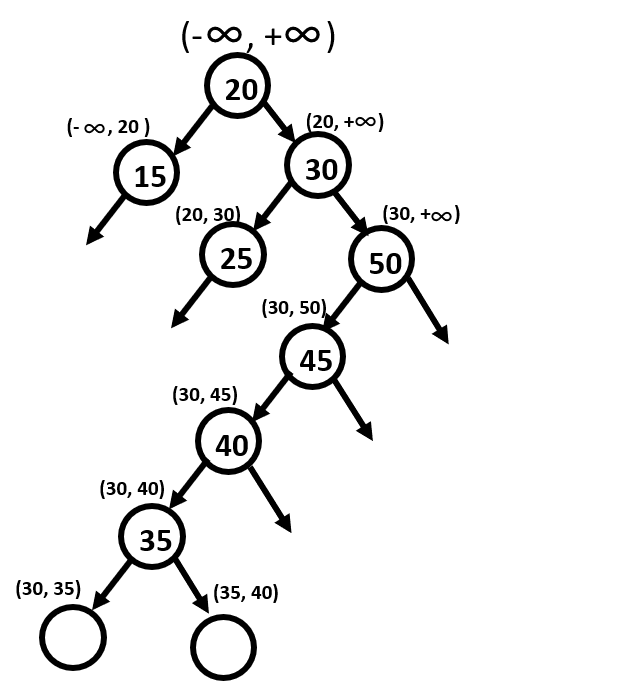
\includegraphics[width=70mm,scale=0.5]{FIG/range_prop.png}
\caption{An example of BST with each node labeled with \emph{range}; lower and upper bound for a key}
\label{range_bst}
\end{figure}
The range for root node is always $(-\infty,+\infty)$ and then, we can calculate the range for all nodes in the tree by enforcing each node to propagates appropriate bounds. For the left child, range will be lower-bound for the node (lower-bound) and the key in the node (upper-bound), while for the right child range will be a key in the node (lower-bound) and upper-bound for the node (upper-bound). This properties in each node help us to prove that the thread have changed the state of data-structure to the valid state. For instance, we can confirm that a key has been inserted in the right place if a key is inside the range of the node. Suppose we want to insert a key $38$ in \ref{range_bst}, then we will locate \emph{right} child of $35$ as the right place for $38$. During insertion, we can confirm that the node is indeed right place for $38$ by checking that $38$ is in the range (35,40). We introduce the $range$ in our proof using the ghost variables. This $ranges$ along with other information about the node represent the abstract state of the data structure. We have used two kind of ghost state in our proof: \emph{per-node} ghost state and \emph{overall} ghost state.\\
\textbf{Per-node Ghost State}: The per-node ghost state is includes a node's range and other information about the node: its current key, value, and ghost names of its child nodes. In VST, we can use a type as ghost state by proving an instance of the \texttt{Ghost} typeclass, analogous to the \emph{resource algebras} of Iris. The essential part is a \emph{join} relation describing how two pieces of ghost state combine. We define the join of two ranges to be the range that contains both of them, and use an \emph{exclusive} algebra for the rest of the data, so that only one thread knows the current state of a node at a time. 
Ghost state is shared between the per-node lock invariants and the abstract state of the data structure using the \emph{reference} pattern: each thread holds partial information describing its contribution to the shared state, and the shared resources hold a ``reference'' copy that records all of the contributions. In VST, this is implemented with assertions $\mathsf{my\_half}\ g\ \mathit{sh}\ a$ and $\mathsf{public\_half}\ g\ r$, where $g$ is the node's identifier ($\gnamety$), $a$/$r$ is the value of the ghost state, and $\mathit{sh}$ is a share describing how much of the reference value is known: if $\mathit{sh}$ is the full share, then we know that $a = r$. In the proof, the \texttt{my\_half} assertion for a node will be held by the node's lock, and \texttt{public\_half} will be held by the shared state.

\textbf{Overall Ghost State}: We now have per-node ghost state for each node, indexed by a ghost name $g_n$. But if we are given an arbitrary $\gnamety$ for a node, we do not know whether that $\gnamety$ exists in the tree. We need another kind of ghost state to hold the set of all nodes in the current tree. Again we can use the ``reference'' pattern to define this ghost state, where the abstract state $\mathsf{ghost\_ref}\ s$ holds the full set of nodes, and each node's lock invariant holds an $\mathsf{in\_tree\ g_n}$ assertion guaranteeing that $g_n$ is in $s$.%notation for gnames
\ignore{\begin{verbatim}
Definition ghost_ref g r1 := ghost_reference(P := set_PCM) r1 g.
Definition in_tree g g1 := EX sh: share, ghost_part(P :=set_PCM) sh (Ensembles.Singleton g1) g.
\end{verbatim}}
\ignore{The global invariant, which we introduced in our atomic specification as the $\treerep$ predicate above, ties together the pieces as follows:
\begin{align*}\treerep(T,g) \triangleq *_n. \mathsf{public\_half\textsubscript{gn}} \ (\mathit{range}_n* \mathit{ghost\_info}_n)\ ] *\ \mathsf{ghost\_ref}\ g\ \{ gn\  \} \end{align*}
 Later while writing atomic specification, we will use $\mathsf{ghost\_ref}$ and $\mathsf{in\_tree}$ in the public and private part respectively. Once we open \emph{global invariant}, we get access to $\mathsf{ghost\_ref}$ which will be used with $\mathsf{in\_tree}$ to establish the fact that node actually exists in the tree. We proved the following lemma for this:
$$
Lemma\ \mathbf{\ node\_exist\_in\_tree : }\ \forall\ g\ s\ g\_in,\  \mathbf{in\_tree}\ g\ g\_in  * \mathbf{ghost\_ref}\ g\ s\ \Rightarrow\ g\_in\ \in s .
$$}
\subsubsection{Handle and Abstract State}
Now we are ready to define the $\treerep$ and $\nodeboxrep$ predicates.

describe lock invariant

We combine pieces of information discussed above, \emph{recursive lock invariant} from \ref{safety} and \emph{ghost states}, to write the atomic specification. The private pre- and postcondition of the atomic specification is given by defining the predicate $\nodeboxrep(p,g,g\_root)$ that describes the concrete state of the BST along with the contribution part of the both kind of ghost states explained above.The root node $p$ is represented by ghost name $g\_root$ and overall ghost state is represented by ghost name $g$. The $\nodeboxrep$ predicate ties together $\mathsf{my\_half}$ part of per-node ghost state and $\mathsf{in\_tree}$ of over-all ghost state inside the $\mathsf{lock\_inv}$ assertion of each node's lock as follows:
\begin{align*}
    &\nodeboxrep_{\pi}(p,g,g\_root) \triangleq  p\mapsto\ (lock,tp)\ *\ \mathsf{lock\_inv_{\pi}}(lock, \mathsf{selflock}_{0.5}(lock,R))) \\&R  \triangleq\ \ghost{\mathsf{my\_half}(range,info)}{g\_root}\ *\ \ghost{\mathsf{in\_tree}\ (g\_root)}{g}\ *\ \exists\ pa\ pb\ ga\ gb,\ tp\mapsto\ (pa * pb)\ *\  \nodeboxrep_{0.5}(pa,g,ga) \\& *\ \nodeboxrep_{0.5}(pb,g,gb))\end{align*}
    
The public pre- and postcondition of the atomic specification is given by defining the predicate $\treerep(T,g)$ that describes the abstract state of the binary search tree $T$  in terms of collection of ghost states each describing the information about separate node in the tree.. The $\treerep$ predicate ties together $\mathsf{public\_half}$ part of per-node ghost states and $\mathsf{ghost\_ref}$ of over-all ghost state as follows: \begin{align*}&\mathsf{ghost\_tree\_rep}(tg,range, g, g\_current) \triangleq\ \exists\ k, v, ga, gb\ \in tg,\ghost{\mathsf{public\_half}\ (range, Some(k,v,ga,gb))}{g\_current}\\& *\ \mathsf{ghost\_tree\_rep}(left(tg),(left(range),k),g,ga)\ *\ \mathsf{ghost\_tree\_rep}(right(tg),(k, right(range)),g,gb) \end{align*}
\begin{align*}\treerep(T,g,g\_root) \triangleq \ \exists\ (tg:ghost\_tree),\ &\mathsf{pure\_tree}(tg)\ =\ T\ \land\ \mathsf{ghost\_tree\_rep}(tg,(-\infty, +\infty),g,g\_root)&\\ *\ \ghost{\mathsf{ghost\_ref}\ (\mathsf{find\_ghost\_set}(tg))}{g}\end{align*}
Where $tg$ is called \emph{ghost tree}, which can be existentially quantified, extend the node in pure tree $T$ with actual pointer and ghost names for child nodes. 

The atomic specification for any binary search tree's operation \texttt{op} should then be
\begin{align*}\forall t.\ \langle \nodeboxrep(p,g,g_{\mathit{root}})\ |\ \treerep(t,g)\rangle\ \texttt{op}(p)\ \langle \nodeboxrep(p,g,g_{\mathit{root}})\ |\ \treerep(t', g)\rangle
\end{align*}
where $t$ and $t'$ are the abstract state of a tree before and after the function's execution. Now we are prepared to prove that each of our BST functions satisfies its specification.

\subsection{Insert and Lookup}

\subsubsection{insert}
The C outline-code for the insert method of binary search tree is shown in \ref{insert}. A node has a lock, key, value, and pointers to the left and right child. Each leaf node in tree are empty node with lock. Whenever a thread try to insert key-value pair in the tree, it first spans the tree to find the right position for new key using hand-over-hand locking mechanism; acquire the lock for child before releasing the lock for node. After locating right leaf node to insert new key-value, thread creates two new empty leaf nodes, insert key-value in the current node, and link the newly created leaf nodes to the current node. If the key already exist in the tree, then thread simply swaps the old value associated with node with the new value keeping the child pointers as it is.

The atomic specification for insert method can be written as follows:
$$\forall t.\ \langle \nodeboxrep(p,g,g\_root)\ |\ \treerep(t,g)\rangle $$ 
$$\texttt{insert}(p,k,v)$$
$$\langle \nodeboxrep(p,g,g\_root)\ |\ \treerep(t[k\mapsto v],g)\rangle $$
We are not guaranteed that the state of  a tree at the end of the insertion will be $t[k\mapsto v]$ where $t$ is the tree state when insert is called; rather, we know that p always holds some tree during the function's execution, and at some point the function will take that tree $t$, add $[k\mapsto v]$, and then eventually return, while in the meantime another thread may have modified the state of tree from $t[k\mapsto v]$ to any other arbitrary state that the current thread do not know.

Since we have given the specification that is strong enough to specify both the safety and the functional correctness properties of insert method, we can now verify that body of the function satisfies the atomic specification given above using various VST and Iris (encoded in VST) tactics. Once we have outermost specification for a function, the another creative part in verification is finding the right loop-invariant. We defines the loop invariant for the insert function as follows: 
\begin{align*} &\mathsf{insert\_inv}(b, x, g, g\_root) \triangleq\ \exists\ \mathit{lock},\mathit{g\_current},\mathit{np},\mathit{range},\mathit{info},\ (x\in \mathit{range})\ \land \ \ghost{\mathsf{my\_half}(\mathit{range},\mathit{info})}{g\_current}\ *\ R\ \mathit{np}\\& * \mathsf{lock\_inv}(\mathit{lock},\mathit{lsh2},R')\ *\ \nodeboxrep(b,g,\mathit{g\_root})\ *\ \mathsf{atomic\_shift} (P_p,E_i,E_o,Q_p,Q) \end{align*}   

Where $\mathsf{P_p}$ and $\mathsf{Q_p}$ are $\treerep(t,g)$ and $\treerep(t[k\mapsto v],g)$ respectively. The resources $\mathsf{R}$, parameterized by a node pointer $np$, describes the concrete information about a node. Also, $x$ is the key to be inserted that must be in the bound $\mathsf{range}$.  This loop invariant has some existential variables which characterized the state of each iteration of loop in the C code.

Figure \ref{insertproof} shows the $\texttt{insert}$ function annotated with separation logic specification. The proof starts with $\nodeboxrep$ and $\mathsf{atomic\_shift}$ as the precondition. After acquiring the lock for the root node, the thread accesses the information inside the lock invariant of the root node. In order to prove $\mathsf{while}$ loop, we show that the precondition satisfies the $\mathsf{insert\_inv}$, then prove that the loop body preserves the loop invariant ( cases inside $\mathsf{else if}$ clauses at line 15 and 17 in \ref{insert}).   Once we locate the empty node for inserting new key-value pair (i.e inside the first $\mathsf{if}$ clause), we open the global invariant encoded in the $\mathsf{atomic\_shift}$, create the ghost names $\texttt{g1}$ and $\texttt{g2}$ for two new empty child nodes of current node, and prove that insertion satisfy the public postcondition $\treerep(t[k\mapsto v],g)$ with the help of $\mathsf{sync\_commit}$ rule described in section \ref{atomicity}. This is the \emph{linearization point} of the $\mathsf{insert}$ operation and must be done at any point in the proof, but before releasing the current node's lock (i.e in critical section). In order to prove the public postcondition $\treerep(t[k\mapsto v],g)$, we need to first locate the current node in $\treerep(t,g)$ using ghost name $g\_current$, and then perform necessary modification such that the final state of the global invariant satisfies $\treerep(t[k\mapsto v],g)$. We create and prove separate lemma for this, called $\emph{extract}$ lemma which is depicted in the \ref{extract_insert}.  

With the help of $\mathsf{in\_tree}$ assertion, we locate a leaf node denoted by ghost name $g\_current$ in the global state $\treerep(t,g)$. Then we prove the \emph{extract} lemma, which says that the state of tree after adding new key-value pair (k,v) will be $\treerep(t[k\mapsto v],g)$, by applying induction in $t$. 

Another important step in the $\mathsf{insert}$ proof is the case when we find that the key to be inserted already exists in the tree (i.e. the last $\texttt{else}$ clause in C code). The modification of the global state of the tree t is shown in \ref{extract_insert2}. In that case, the old value $v'$ associated with key is overridden by new value $v$ keeping a key $40$ and child pointers as as they are. This is also the \emph{linearization point} of the $\mathsf{insert}$ operation. We augment the same $\emph{extract}$ lemma with the clause that states the scenario in \ref{extract_insert2}, and prove the lemma in the same induction over the tree $t$.

In the rest two cases, the $\texttt{insert}$ method compares the key
of the current node with the key $\texttt{x}$ and goes down into the
corresponding left or right branch. We need to show that the range in
the ghost state shrinks correctly. To achieve this goal we open the
global invariant encoded in the $\mathsf{atomic\_shift}$ to retrieve
the necessary information. But this time these operations maintain the
original state. For the left branch case, we accomplish the proof by
the following lemma:
%\begin{verbatim}
%Lemma in_tree_left_range:
%  forall (B: Type) (b: tree -> B -> mpred) (Q : B → mpred) (x x0: Z) (g g_root : gname)
%    (inv_names : invG) (v: val) (g_in ga gb: gname) (r a: node_info),
%    check_key_exist' x r.1 = true -> r.2 = Some (Some (x0, v, ga, gb)) -> x < x0 ->
%    atomic_shift (λ BST : tree, !! sorted_tree BST && tree_rep2 g g_root BST) ∅ ⊤
%                 b Q * my_half g_in gsh1 r * in_tree g g_in * my_half ga gsh1 a
%    |-- atomic_shift (λ BST : tree, !! sorted_tree BST && tree_rep2 g g_root BST) ∅ ⊤
%    b Q * my_half g_in gsh1 r *
%    (EX ba, !! (less_than_equal ba r.1.1 = true /\
%                range_inclusion a.1 (ba, Finite_Integer x0) = true) &&
%            (in_tree g g_in * my_half ga gsh1 (ba, Finite_Integer x0, a.2))).  
%\end{verbatim}
The lemma for the right branch case is similar. Both use the
$\texttt{sync\_rollback}$ lemma described in section \ref{atomicity}.
  
\begin{figure}[htb]
\centering
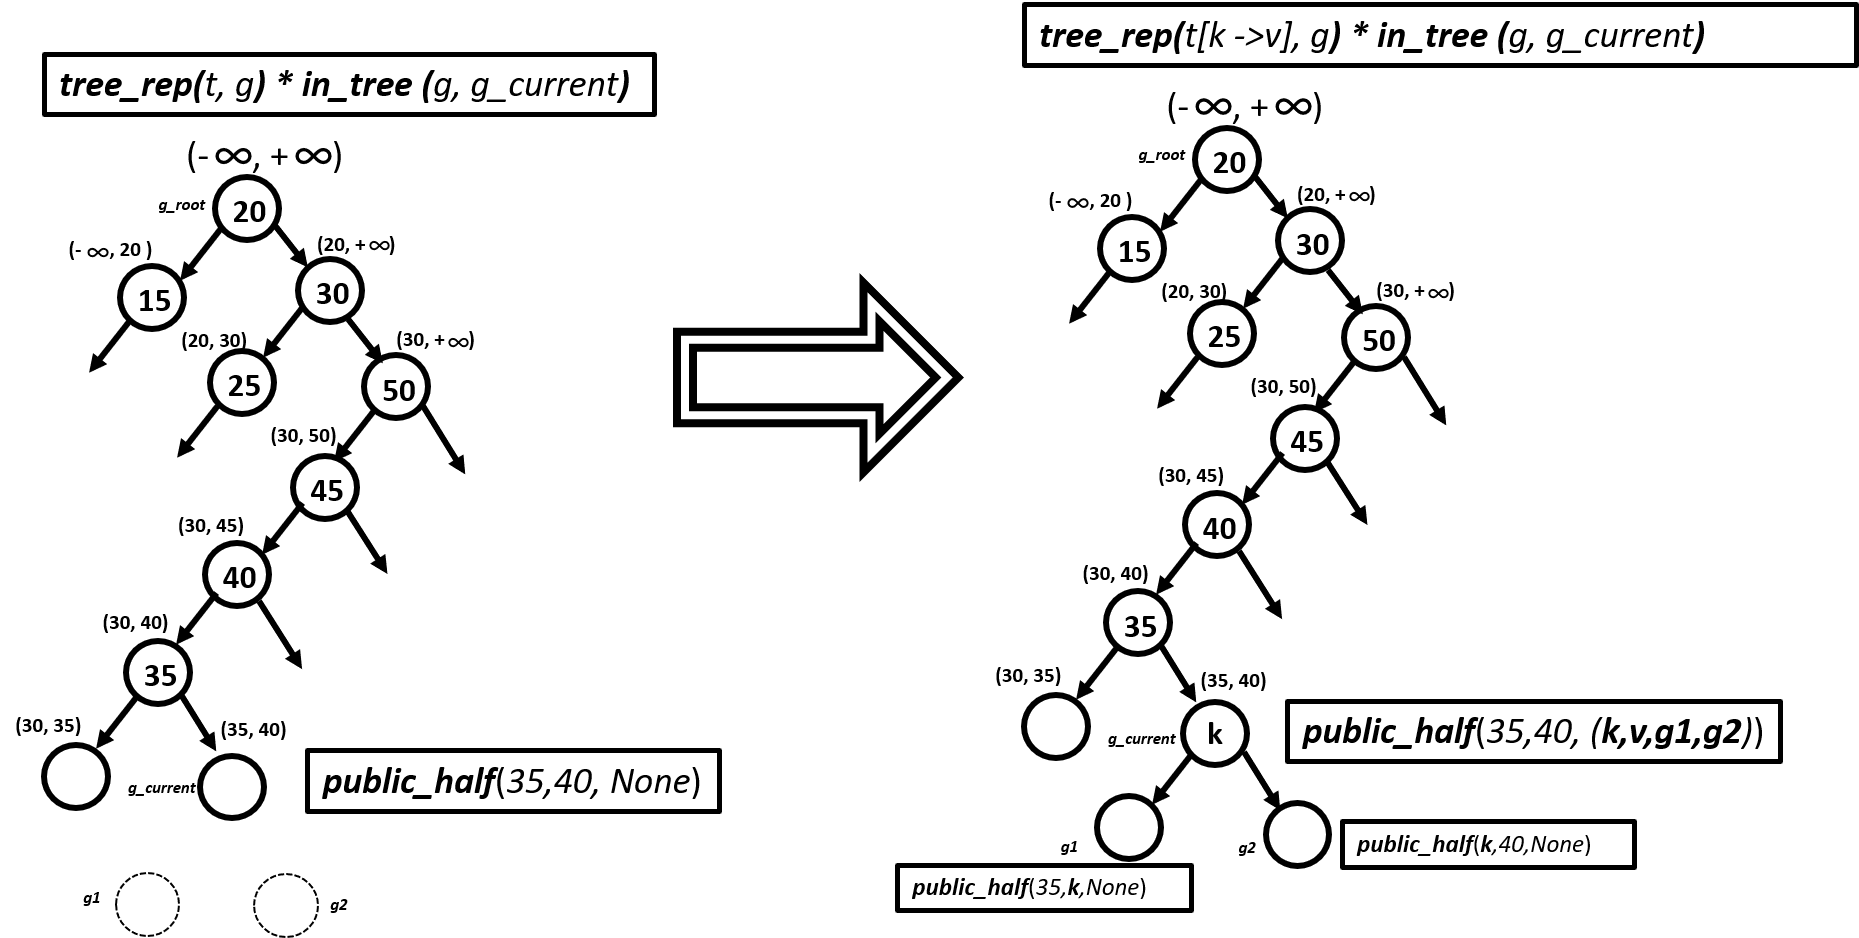
\includegraphics[width=150mm,scale=0.5]{FIG/extract_insert.png}
\caption{A visual depiction of the change in global state of BST during $\mathsf{insert(k,v)}$ operation }
\label{extract_insert}
\end{figure}
\begin{figure}[htb]
\centering
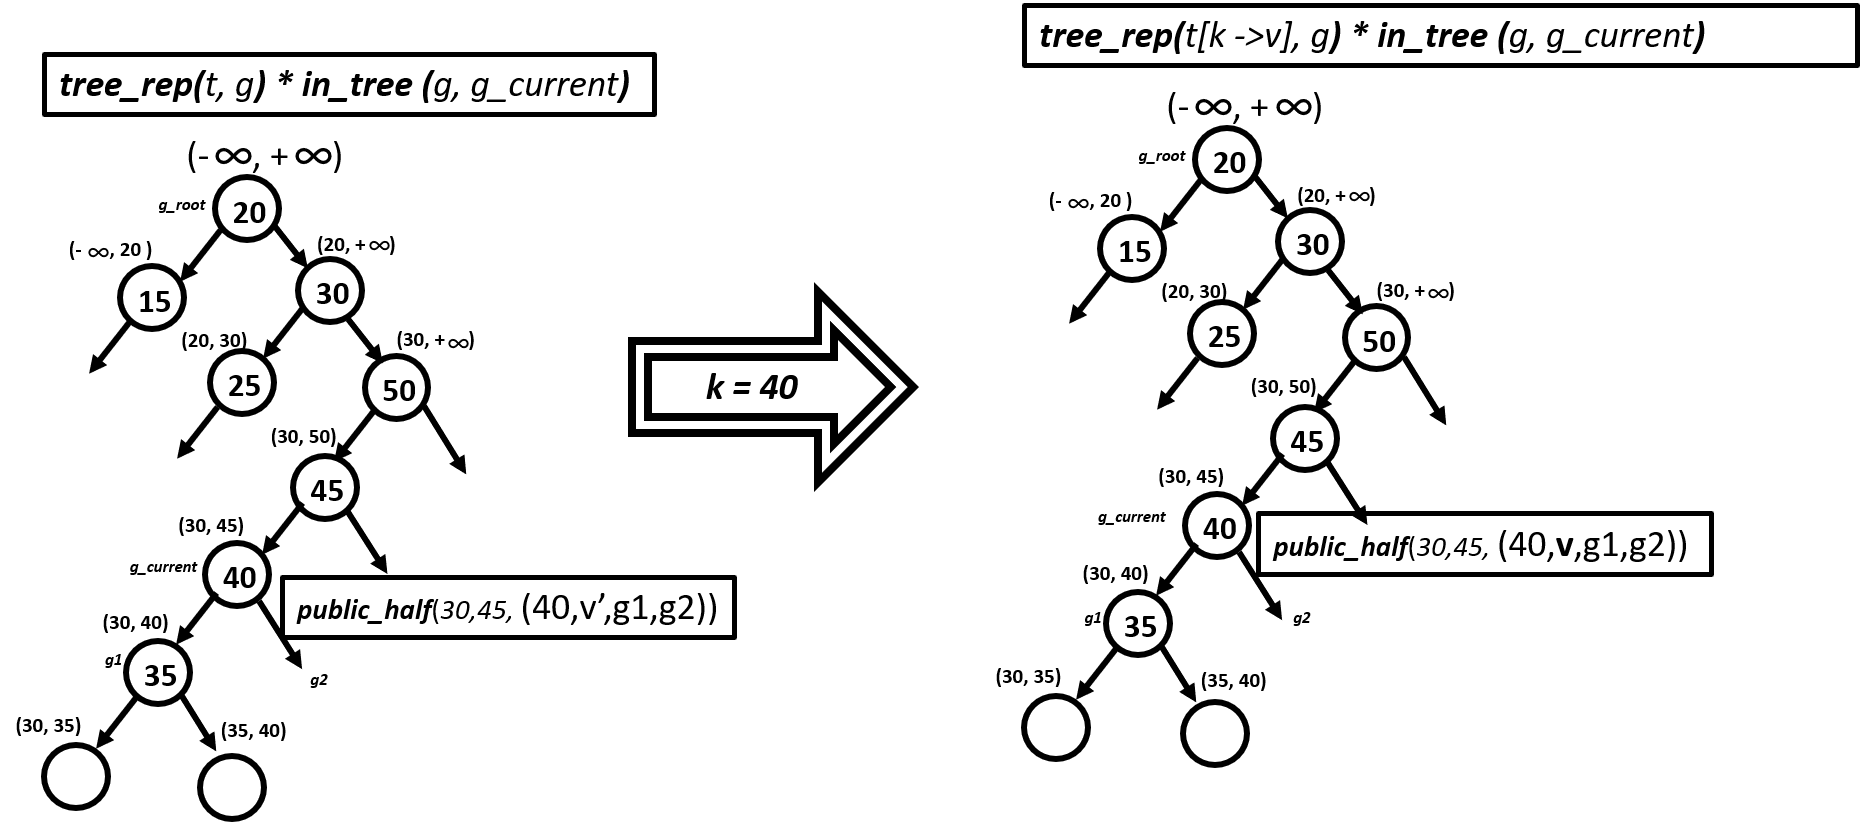
\includegraphics[width=150mm,scale=0.5]{FIG/extract_insert_2.png}
\caption{A visual depiction of the change in global state of BST during $\mathsf{insert(k,v)}$ operation, where key $k$ already exists in the tree $t$ }
\label{extract_insert2}
\end{figure}
\begin{figure}[htp]
\begin{subfigure}[t]{1\textwidth}
 $$\left\{\begin{array}{l} \nodeboxrep(b,g\_root)\ *\ \mathsf{atomic\_shift}(P_p,E_i,E_o,Q_p,Q)\end{array}\right\}$$
 \vspace*{-20pt}
\begin{lstlisting}[language = C,numbers = none]
insert(treebox t, int x, void *value)
  tree_t *tgt = *t;
  acquire(tgt->lock)
 \end{lstlisting}  
 $$\left\{\begin{array}{l} \ghost{\mathsf{my\_half}((-\infty,+\infty),info)}{g\_root}\ *\ R\ b\ *\ \mathsf{lock\_inv}(lock,lsh2,R')\ *\ \\
 \nodeboxrep(b,g\_root)\ *\ \mathsf{atomic\_shift}(P_p,E_i,E_o,Q_p,Q)\end{array}\right\} \Rrightarrow \left\{\begin{array}{l} insert\_inv \end{array}\right\}$$ 
  \begin{lstlisting}[language = C,numbers = none]
  for(;;) {
       \end{lstlisting}   
   $$\left\{\begin{array}{l} insert\_inv \end{array}\right\} \triangleq \left\{\begin{array}{l}(x\in range)\land \ghost{\mathsf{my\_half}(range,info)}{g\_current}*\ R\ np\ \\*\mathsf{lock\_inv}(lock,lsh2,R')\ *\ \nodeboxrep(b,g\_root)\ *\ \mathsf{atomic\_shift}(P_p,E_i,E_o,Q_p,Q)\end{array}\right\}$$
      \begin{lstlisting}[language = C,numbers = none]
    p = tgt->t;
    if (p==NULL)
      tree_t *p1, *p2 = malloc();
      p = malloc(); tgt->t = p;
      p->key=x; p->value=value; p->left=p1; p->right=p2;
           \end{lstlisting} 
  $$\left\{\begin{array}{l} \ghost{\mathsf{own}\ (a1)}{g1}\ *\ \ghost{\mathsf{own}\ (a2)}{g2}\ *\ \ghost{\mathsf{my\_half}(range,None)}{g\_current}*\ R\ np\ \\*\mathsf{lock\_inv}(lock,lsh2,R')\ *\ \nodeboxrep(b,g\_root)\ *\ \mathsf{atomic\_shift}(P_p,E_i,E_o,Q_p,Q)\end{array}\right\} \Rrightarrow{\textbf{sync\_commit}}$$
$$\left\{\begin{array}{l} \ghost{\mathsf{my\_half}(range,None)}{g\_current}*\ R\ np\ *\mathsf{lock\_inv}(lock,lsh2,R')\ *\ \nodeboxrep(b,g\_root)\ *\ Q\end{array}\right\}$$
 \vspace*{-10pt}
        \begin{lstlisting}[language = C,numbers = none]
      release2(l);
         \end{lstlisting}
       $$\left\{\begin{array}{l} \nodeboxrep(b,g\_root)\ *\ Q\end{array}\right\}$$
        \vspace*{-10pt}
         \begin{lstlisting}[language = C,numbers = none]
      return;
     else 
        ....
       else 
      	p->value=value;
      	\end{lstlisting} 
$$\left\{\begin{array}{l} \ghost{\mathsf{my\_half}(range,None)}{g\_current}*\ R\ np\ *
\mathsf{lock\_inv}(lock,lsh2,R')\ *\ \\\nodeboxrep(b,g\_root)\ *\ \mathsf{atomic\_shift}(P_p,E_i,E_o,Q_p,Q)\end{array}\right\} \Rrightarrow{\textbf{sync\_commit}}$$
$$\left\{\begin{array}{l} \ghost{\mathsf{my\_half}(range,None)}{g\_current}*\ R\ np\ *\mathsf{lock\_inv}(lock,lsh2,R')\ *\ \nodeboxrep(b,g\_root)\ *\ Q\end{array}\right\}$$
         \vspace*{-10pt}
      	\begin{lstlisting}[language = C, numbers = none]
        release2(l);
        \end{lstlisting}
        $$\left\{\begin{array}{l}  \nodeboxrep(b,g\_root)\ *\ Q\end{array}\right\}$$
         \vspace*{-10pt}
        \begin{lstlisting}[language = C, numbers = none] 
      	return;
\end{lstlisting}
\end{subfigure}
\caption{The $\texttt{insert}$ function annotated with separation logic specification}
\label{insertproof}
\end{figure} 


\subsubsection{lookup}

The code for the $\mathsf{lookup}$ method is shown in Figure
\ref{lookupproof}. It takes the location of the root pointer and a key
as the arguments. A thread spans the tree to find a given key using
hand-over-hand locking mechanism. Once a thread finds the key in the
tree, it gets the value associated with that key, release the current
node's lock, and return the value.

The atomic specification for $\mathsf{lookup}$ method can be written
as follows:
\begin{align*} \forall M.\ \langle &\nodeboxrep(p,g,g\_root)\ |\ \treerep(M,g,g\_root)\rangle \end{align*} 
$$\mathsf{lookup}(p,k)$$ 
\begin{align*}\langle\lambda v.\ \nodeboxrep(p,g,g\_root)\ |\ (v = M[k])\ \wedge\ \treerep(M,g,g\_root)\rangle \end{align*}

This specification is quite similar to the specification given to the
$\mathsf{insert}$ method, except the content of public part in the
postcondition. It says that at some point the $\mathsf{lookup}$
function will take a map $M$, get the value $M[k]$, and then
eventually return with the value. Again, it is not guaranteed that the
state of the map at the end of the execution is the same one when the
$\mathsf{lookup}$ is called. The key part to verify the specification
is to prove the loop inside the $\mathsf{lookup}$ method. We define
the loop-invariant as follows:
\begin{align*} &\mathsf{lookup\_inv}(b, x, \mathit{g\_root}, \mathit{range},\mathit{info}) \triangleq\ \exists\ \mathit{lock},\ \mathit{g\_current},\ \mathit{np},\ (x\in \mathit{range})\ \land \ \ghost{\mathsf{my\_half}(\mathit{range},\mathit{info})}{\mathit{g\_current}}\\& *\ R\ np\ * \mathsf{lock\_inv}(\mathit{lock},\mathit{lsh2},R')\ *\ \nodeboxrep(b,\mathit{g\_root})\ *\ \mathsf{atomic\_shift} (P_p,E_i,E_o,Q_p,Q) \end{align*}

Where $P_p$ and $Q_p$ are $\treerep(g\_root, t)$ and $(v =
M[k])\ \wedge\ \treerep(g\_root, t)$ respectively. The proof steps for
the $\texttt{lookup}$ verification are almost similar to the steps
used in $\texttt{insert}$ verification with a few differences which we
discuss below.


Figure \ref{lookupproof} shows the $\mathsf{lookup}$ function
annotated with separation logic specification. The proof starts with
$\nodeboxrep$ and $\mathsf{atomic\_shift}$ assertions as the
precondition and follows the approach similar to the $\mathsf{insert}$
proof for the verification of loop body. Once we find the given key
(i.e. the last $\mathsf{else}$ clause in C code) in the tree, we need
to confirm that the current state of the tree in the global invariant
agrees with the fact that the current node, represented by
$\texttt{g\_current}$ in the global invariant, actually contains the
key-value pair $(k, v)$ in the ghost state represented
$\texttt{g\_current}$. We accomplish this by opening the global
invariant encoded in the $\mathsf{atomic\_shift}$, and proving that
lookup satisfy the public postcondition $\mathsf{Q\_p}$ with the help
of the $\mathsf{sync\_commit\_same}$ lemma described in section
\ref{atomicity}. This is the \emph{linearization point} of the
$\mathsf{lookup}$ operation and must be done before releasing the
current node's lock. In the case of spanning left or right sub-tree,
we need to establish $\mathsf{lookup\_inv}$ at the end $\mathsf{if}$
and $\mathsf{else\ if}$ clause. Here, we need to show that the key we
are searching is still in the bound for left/right node, so we use
$\mathsf{sync\_rollback}$ lemma to extract the bound of a left/right
node encoded as the ghost state in the public precondition
($\treerep(M, g, g\_root)$).

A critical difference from $\texttt{insert}$ is that the
$\texttt{lookup}$ method does not change the shape the tree. With the
help of the $\texttt{sync\_commit\_same}$, we need no longer the
heavyweight $\emph{extract}$ lemma but instead a simpler
$\emph{ramif}$ lemma to locate the current node in the global
invariants:
\begin{verbatim}
Lemma ghost_tree_rep_public_half_ramif: forall tg g_root r_root g_in,
Ensembles.In (find_ghost_set tg g_root) g_in -> ghost_tree_rep tg g_root r_root |-- 
EX r: node_info, !! (range_info_in_tree r r_root tg) && (public_half g_in r * 
(public_half g_in r -* ghost_tree_rep tg g_root r_root)).
\end{verbatim}

\begin{figure}[htp]
\begin{subfigure}[t]{1\textwidth}
 $$\left\{\begin{array}{l} \nodeboxrep(b,g\_root)\ *\ \mathsf{atomic\_shift}(P_p,E_i,E_o,Q_p,Q)\end{array}\right\}$$
\begin{lstlisting}[language = C,  numbers = none]
void *lookup (treebox t, int x) {
  struct tree *p; void *v;  struct tree_t *tgt;
  tgt = *t;  void *l = tgt->lock;
  acquire(l);  p = tgt->t;
 \end{lstlisting}  
 $$\left\{\begin{array}{l} \ghost{\mathsf{my\_half}((-\infty,+\infty),info)}{g\_root}\ *\ R\ b\ *\ \mathsf{lock\_inv}(l,lsh2,R')\ *\ \\
 \nodeboxrep(b,g\_root)\ *\ \mathsf{atomic\_shift}(P_p,E_i,E_o,Q_p,Q)\end{array}\right\} \Rrightarrow \left\{\begin{array}{l} lookup\_inv \end{array}\right\}$$ 
  \begin{lstlisting}[language = C, numbers = none]
    while (p!=NULL) {
       \end{lstlisting}   
   $$\left\{\begin{array}{l} lookup\_inv \end{array}\right\} \triangleq \left\{\begin{array}{l}(x\in range)\land \ghost{\mathsf{my\_half}(range,info)}{g\_current}*\ R\ np\ *\\\mathsf{lock\_inv}(lock,lsh2,R')\ *\ \nodeboxrep(b,g\_root)\ *\ \mathsf{atomic\_shift}(P_p,E_i,E_o,Q_p,Q)\end{array}\right\}$$
      \begin{lstlisting}[language = C,  numbers = none]
    if (x<y){
      tgt=p->left;
      ....
    }else if (y<x){
      tgt=p->right;
     ....
    }else {
    v = p->value;
           \end{lstlisting} 
  $$\left\{\begin{array}{l} \ghost{\mathsf{my\_half}(range,info)}{g\_current}*\ R\ np\ *\mathsf{lock\_inv}(lock,lsh2,R')\ *\ \\\nodeboxrep(b,g\_root)\ *\ \mathsf{atomic\_shift}(P_p,E_i,E_o,Q_p,Q)\end{array}\right\} \Rrightarrow{\textbf{sync\_commit\_same}}$$
$$\left\{\begin{array}{l} \ghost{\mathsf{my\_half}(range,info)}{g\_current}*\ R\ np\ *\mathsf{lock\_inv}(lock,lsh2,R')\ *\ \nodeboxrep(b,g\_root)\ *\ Q\end{array}\right\}$$
        \begin{lstlisting}[language = C,  numbers = none]
      release2(l);
         \end{lstlisting}
       $$\left\{\begin{array}{l} \nodeboxrep(b,g\_root)\ *\ Q\end{array}\right\}$$
         \begin{lstlisting}[language = C, numbers = none]
       return v;} }
  release2(l);  return NULL;  }
 \end{lstlisting} 
\end{subfigure}
\caption{The $\texttt{lookup}$ function annotated with separation logic specification}
\label{lookupproof}
\end{figure} 

\subsection{Delete}

\section{Lock-Free BST}
We want to prove that a lock-free BST implementation satisfies the same specification as our hand-over-hand implementation. Unfortunately, provably-correct deletion in a lock-free setting is a research topic in itself (cite?), so we begin with a lock-free BST that only supports insert and lookup. Once again, we want to prove
\begin{mathpar}
\forall t.\ \langle \nodeboxrep\ p\ |\ \treerep\ t\rangle\ \texttt{insert}(p, k, v)\ \langle \nodeboxrep\ p\ |\ \treerep\ (\mathrm{insert}\ t\ k\ v)\rangle

\forall t.\ \langle \nodeboxrep\ p\ |\ \treerep\ t\rangle\ \texttt{lookup}(p, k)\ \langle v.\ \nodeboxrep\ p\ |\ \treerep\ t \land \mathrm{lookup}\ t\ k = v\rangle
\end{mathpar}
though the precise definitions of $\nodeboxrep$ and $\treerep$ will differ. %something about how the fact that the specs are the same really comes across to a client -- and should we prove a client?

\section{Related Work}
\label{related}
Our work is based on the concurrent separation logic of VST in the style of Iris \cite{higherorderghoststate} and the logical atomicity from TaDA logic  \cite{tada}. The notion of the \emph{lower} and \emph{upper} bound is taken from the flow interface paper \cite{krishna2017flow}. Our main technical contributions are the verification of two different implementation of binary search tree (using fine-grained locking and lock-free technique) with respect to the same abstract specification, and first c-level mechanized verification of concurrent search-based data structure (i.e. BST). Most of the other concurrent separation logic (CSL)-based verification works are on toy languages, while VST lets us use the same logic on real C programs. 

Gotsman and Yang \cite{gotsman} is one of the earliest work on concurrent separation logic. They introduced the program logic to reason locally about the heap-manipulating program with the notion of dynamic ownership of heap parts by unbounded number of locks and threads, and shown the verification of singly-linked list with fine-grained locking. Xiong et al. \cite{Xiong2017Abstract} have demonstrated the verification of ConcurrentSkipListMap from java.util.concurrent library using the recent advances in fine-grained concurrency reasoning. Their work is mainly based on the abstract atomicity from TaDa logic, and give two modular specifications for concurrent maps: one specification focus on the entire map structure which is suitable for verifying implementation, and another specification focus on the key-value pairs which appropriate for verifying clients. We use the same idea of atomicity (though implemented in Iris) in our work. 

Krishna et al. \cite{krishna2017flow} have presented the proof technique for concurrent search structure templates based on the flow framework and the Iris separation logic, and verified the implementation of concurrent B-tree, hash tables, and linked lists based on the templates. Their work is closely related to our work; we took some inspiration from them in building our ghost state. But, their proofs are on a toy language rather than real C code.

\section{Conclusion}
\label{conclusion}

%% Bibliography
\bibliography{sources}
\end{document}
